\chapter{Hyperdimensional computing methods\\for amino acid-level predictions}
As discussed in section~\ref{ssec:nlp}, state-of-the-art protein language models primarily rely on transformer-based architectures to learn representations of protein sequences and amino acids in the context of other amino acids. These models have demonstrated their effectiveness in various applications, such as protein function prediction and protein-protein interaction prediction, by capturing complex patterns in amino acid sequences. Moreover, these models are also capable of making detailed predictions at the amino acid level, such as predicting secondary structure. This involves determining local three-dimensional structures of regions within a protein, such as alpha-helices and beta-sheets, based on the sequence of amino acids. This capability further extends their utility in understanding protein structure and function. However, these models are computationally intensive and may be less suitable for certain tasks or scenarios where computational resources are limited.

In section~\ref{sssec:trans}, we explored the idea of encoding information from a residue's neighborhood into a hyperdimensional vector that represents the residue and its surroundings. This approach allows us to capture local sequence information and can serve as an effective encoding scheme for amino acids. To evaluate the effectiveness of this encoding method, we will employ it as an input for several perceptron-based models.

Perceptron-based models, a type of artificial neural network model, have been employed for various machine learning tasks over the years, including classification and regression problems. The perceptron, one of the simplest and earliest types of neural networks, was proposed by Frank Rosenblatt in 1958~\cite{perceptron}. A perceptron consists of a single artificial neuron that receives multiple input features and computes a weighted sum of these inputs. This weighted sum is then passed through an activation function, which determines the output of the perceptron. The learning process involves adjusting the weights of the input features iteratively, using a rule that minimizes prediction errors on the training data. The perceptron learning algorithm starts with an initial set of weights, typically set to zero or small random values. For each instance in the training data, the perceptron computes the output, compares it with the true label, and updates the weights accordingly. The weight update rule is based on the difference between the predicted output and the true label, multiplied by the learning rate and the input feature value. Single-layer perceptrons consist of an input layer and an output layer of perceptrons, allowing for multiclass classifications. However, they can only solve linearly separable problems, limiting their applicability for more complex tasks.

As single-layer perceptrons can only solve linearly separable problems, researchers developed more complex neural network architectures, such as multi-layer perceptrons (MLP), which consist of multiple layers of artificial neurons connected in a feedforward manner. MLPs can learn non-linear patterns in the data by using non-linear activation functions (e.g., sigmoid, tanh, ReLU) and employing backpropagation for weight updates~\cite{mlp}. This enhanced ability to model non-linear relationships allows MLPs to tackle a wider range of problems.

By combining the residue neighborhood encoding method with perceptron-based models, we could develop more computationally efficient alternatives to state-of-the-art transformer-based models. These models may provide valuable insights into protein sequences and amino acids while being more suitable for scenarios with limited computational resources.

\section{Methods}
We used the training dataset compiled by Klausen \textit{et al.} for their model protein language model NetsurfP 2.0~\cite{netsurf} as our training dataset. It contains 10,337 protein sequences obtained from the Protein Data Bank (PDB)~\cite{pdb}. Each residue in these sequences is annotated with its 3- and 8-class secondary structure classification, providing a comprehensive description of the protein's structural properties. The residues have been encoded using our neighborhood-encoder as described in section~\ref{sec:trans} with $n=25$ and $n=100$ using random hyperdimensional vectors for each amino acid. Due to computational memory constraints, we randomly selected 60 \% of the sequences from the original dataset for training and testing (80 \% and 20 \% respectively), ensuring a representative sample of the data.

As for the perceptron-based model, to decrease the computational time, we opted to build, train and evaluate the model in Python due to its support for computations on GPUs on our systems. We employed PyTorch-Lightning v1.8.4 for model construction and training and CUDA v11.7.0 on a high-performance computing (HPC) cluster equipped with an NVIDIA V100 GPU. The model comprised fully-connected layers with an input layer size equal to the dimension of the hyperdimensional vectors (10,000 in this case). Depending on the secondary structure classification desired, the output layer size was set to either 3 or 8. We used a batch size of 128 during training. Between each layer, we incorporated a ReLU (Rectified Linear Unit) activation function to introduce non-linearity into the model. The training loss was monitored using cross-entropy loss, which is well-suited for multi-class classification problems. To optimize the model, we employed the widely-used ADAM optimizer. We evaluated various configurations and hyperparameters to determine the best-performing but still computationally feasible approach:

\begin{table}[h]
    \caption{Overview of model configurations and hyperparameters tested}
    \label{tab:casp3}
    \centering
    \begin{tabular}{l|ccc}
        \toprule
         & Epochs & Learning rate & Size hidden layer(s)\\
        \midrule
        \textbf{SLP} & 100 & 0.03 & /\\
        \hline
        \textbf{1-layer MLP} & 50 & 0.003 & 500\\
        \hline
        \textbf{10-layer MLP} & 200 & 0.0003 & \makecell{8000-5000-2000-1000-800-\\500-200-100-50-20}\\
        \bottomrule
    \end{tabular}
  \end{table}

As test datasets, we opted to use CB513~\cite{cb513} and CASP12~\cite{casp12} (compiled by the developers of NetSurfP 2.0~\cite{netsurf}) since they are easily attainable and commonly used by researchers as benchmark datasets for protein language models. The MLP model with 10 hidden layers was trained using 60 \% of the training data and then evaluated using these test datasets. For extra validation, random dummy data was generated.

\section{Results}
A review of figure~\ref{fig:main8} demonstrates notable issues with the SLP model's ability to train effectively on our dataset. This is signaled by the substantial fluctuations in both loss and validation performance, a trend suggesting an inherent instability in the learning process of this model. Additionally, the 1-layer MLP model also exhibits problematic behavior, as it does not learn as seen in its losscurves in figure~\ref{fig:main83}. tOn top of that, it predicts only one single class during validation (the class with the highest proportion), resulting in a large discrepancy between the accuracy and F1-score. These limitations lead to our decision to discontinue further investigations and experimentation with these particular models.

Figure~\ref{fig:main8e} presents the outcome of the training procedure when applied to 60 \% of the NetSurfP 2.0's training data, with a training-test data split of 0.8-0.2. The model was tested under various conditions, including 3 and 8 secondary structure classifications (denoted as dssp3 and dssp8, respectively), and with a range of hyperdimensional embeddings, developed using neighborhood-encoding ($n = 25$ and $n=100$).

\begin{figure}[htbp]
    \centering
    \begin{subfigure}{0.48\textwidth}
        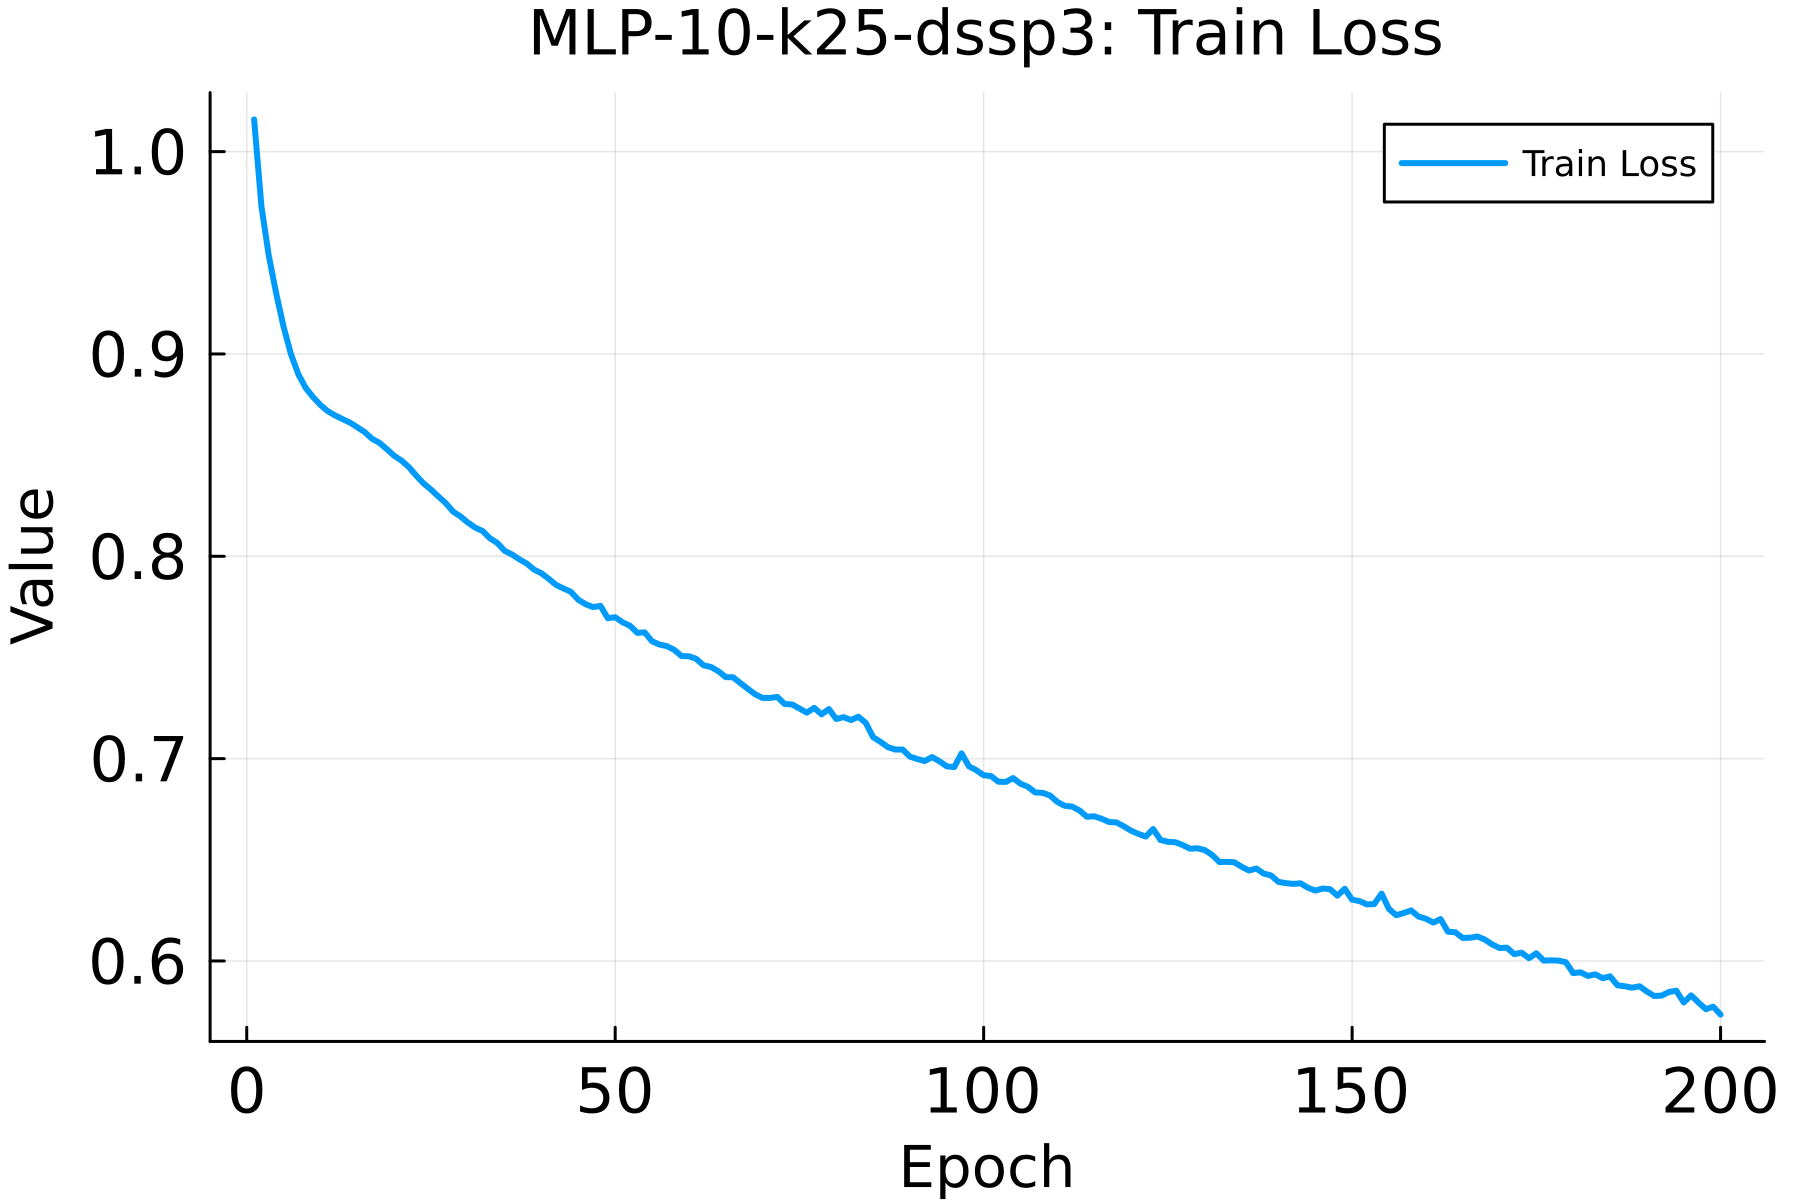
\includegraphics[width=\textwidth]{mlp_fullk25_dssp3_loss}
        \label{fig:subefig}
    \end{subfigure}
    \hfill
    \begin{subfigure}{0.48\textwidth}
        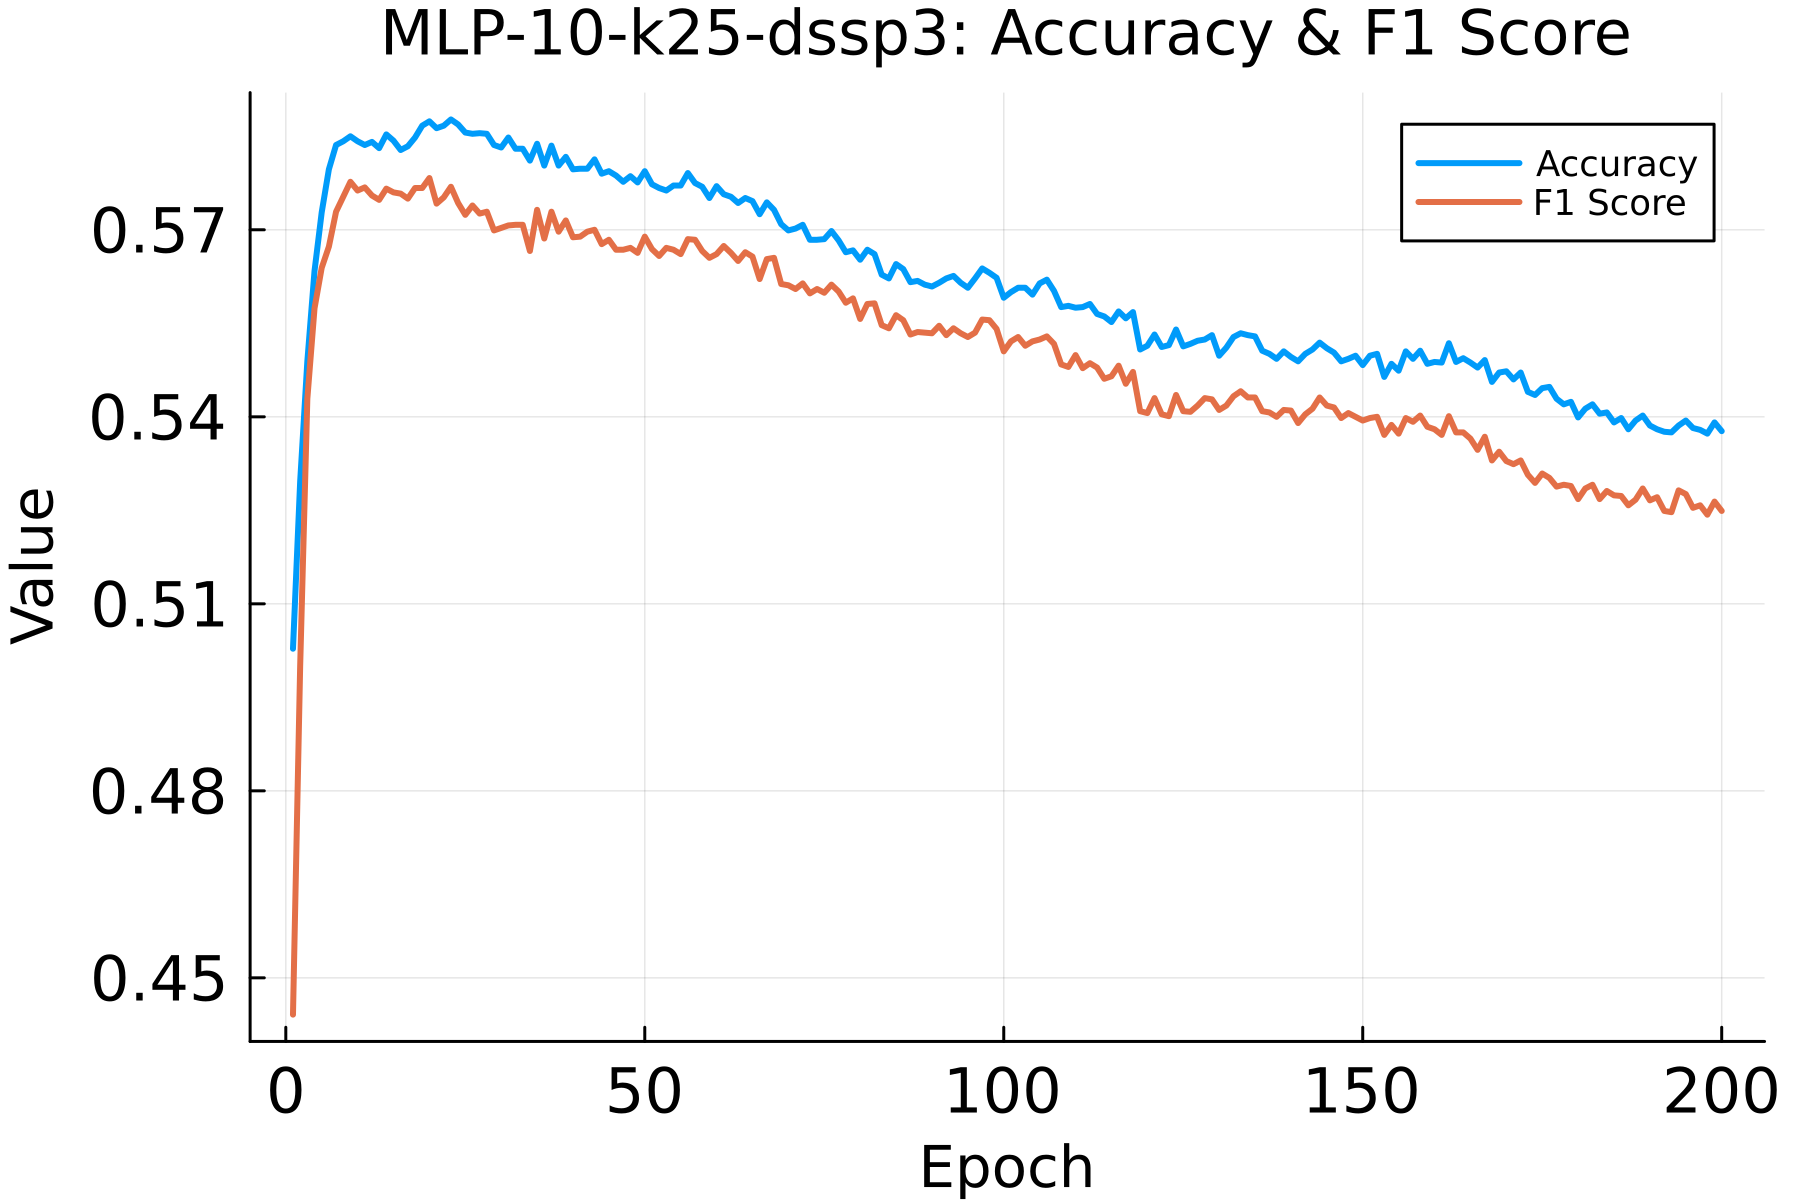
\includegraphics[width=\textwidth]{mlpfull_k25_dssp3_score}
        \label{fig:subefi}
    \end{subfigure}
    
    \begin{subfigure}{0.48\textwidth}
        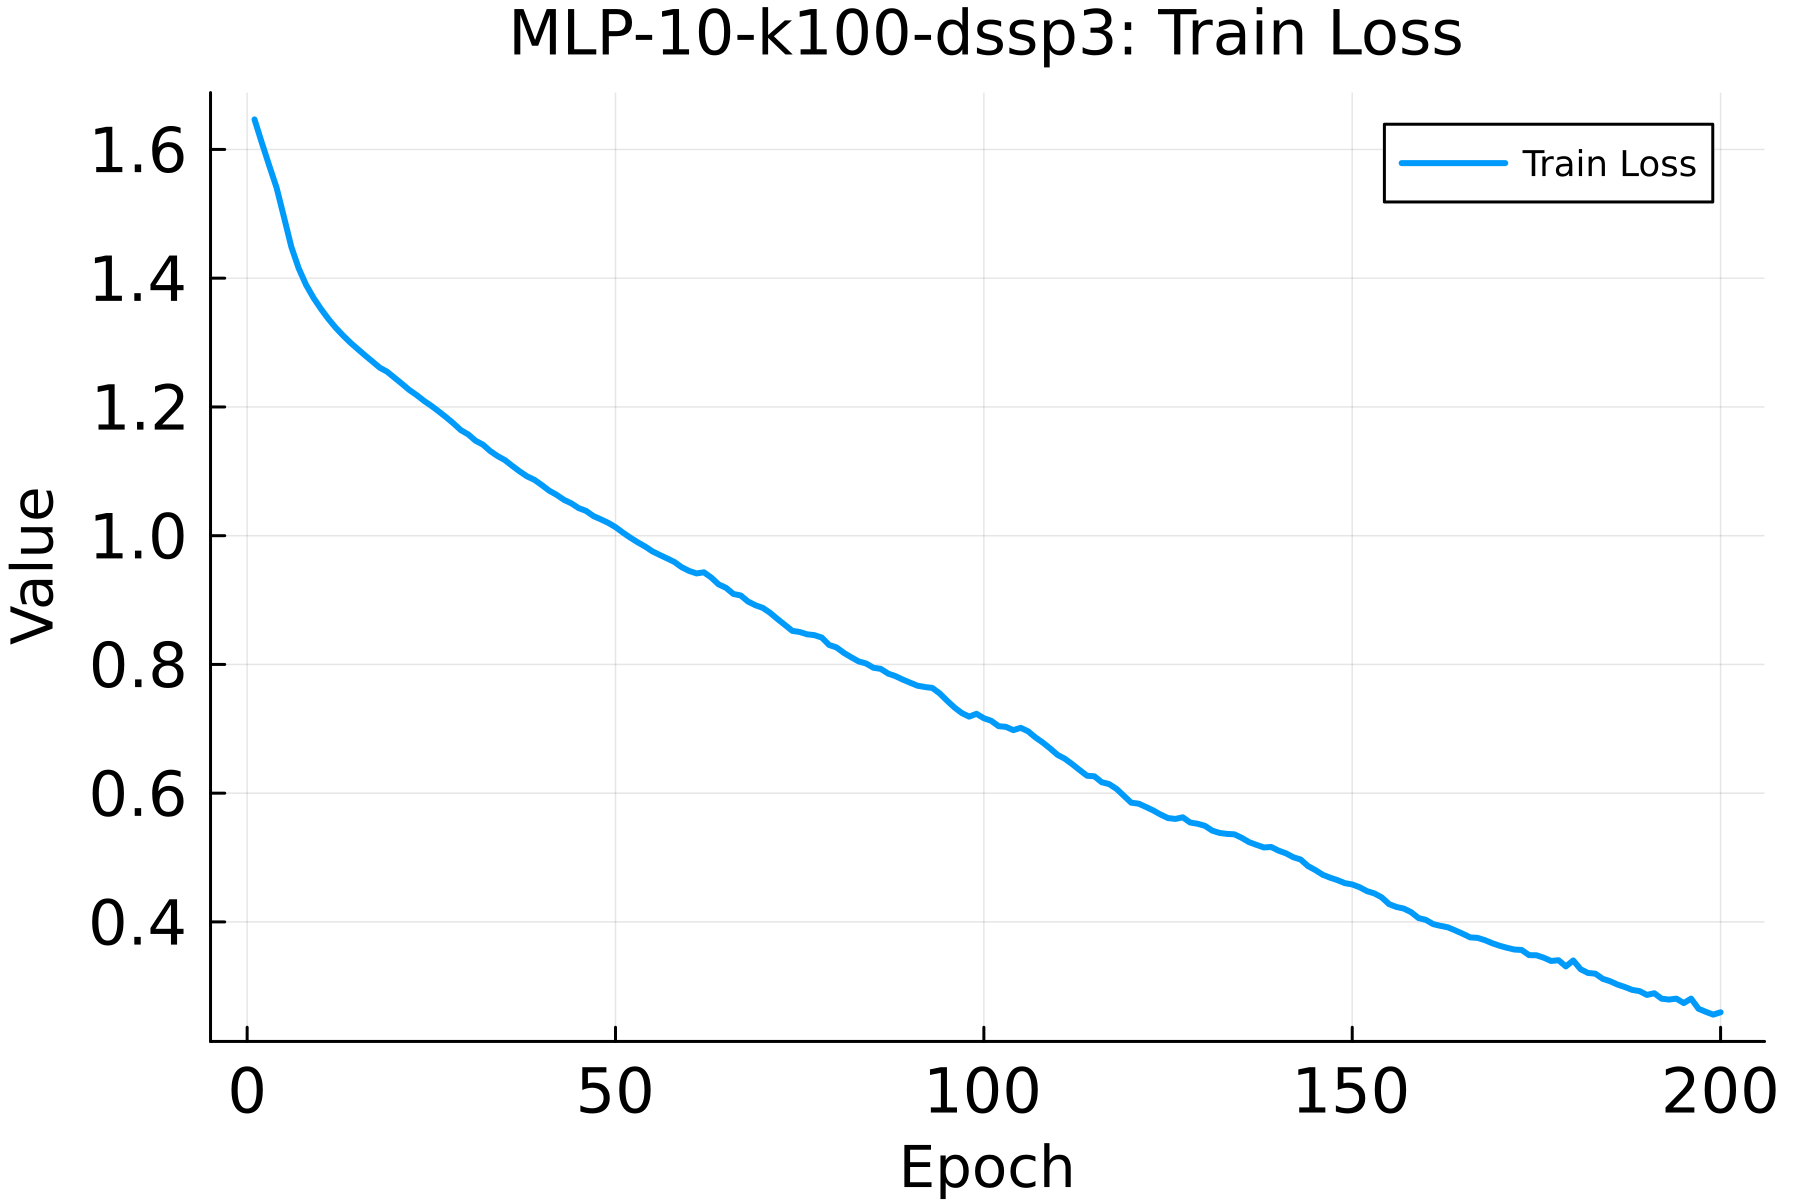
\includegraphics[width=\textwidth]{mlp_fullk25_dssp8_loss}
        \label{fig:subef}
    \end{subfigure}
    \hfill
    \begin{subfigure}{0.48\textwidth}
        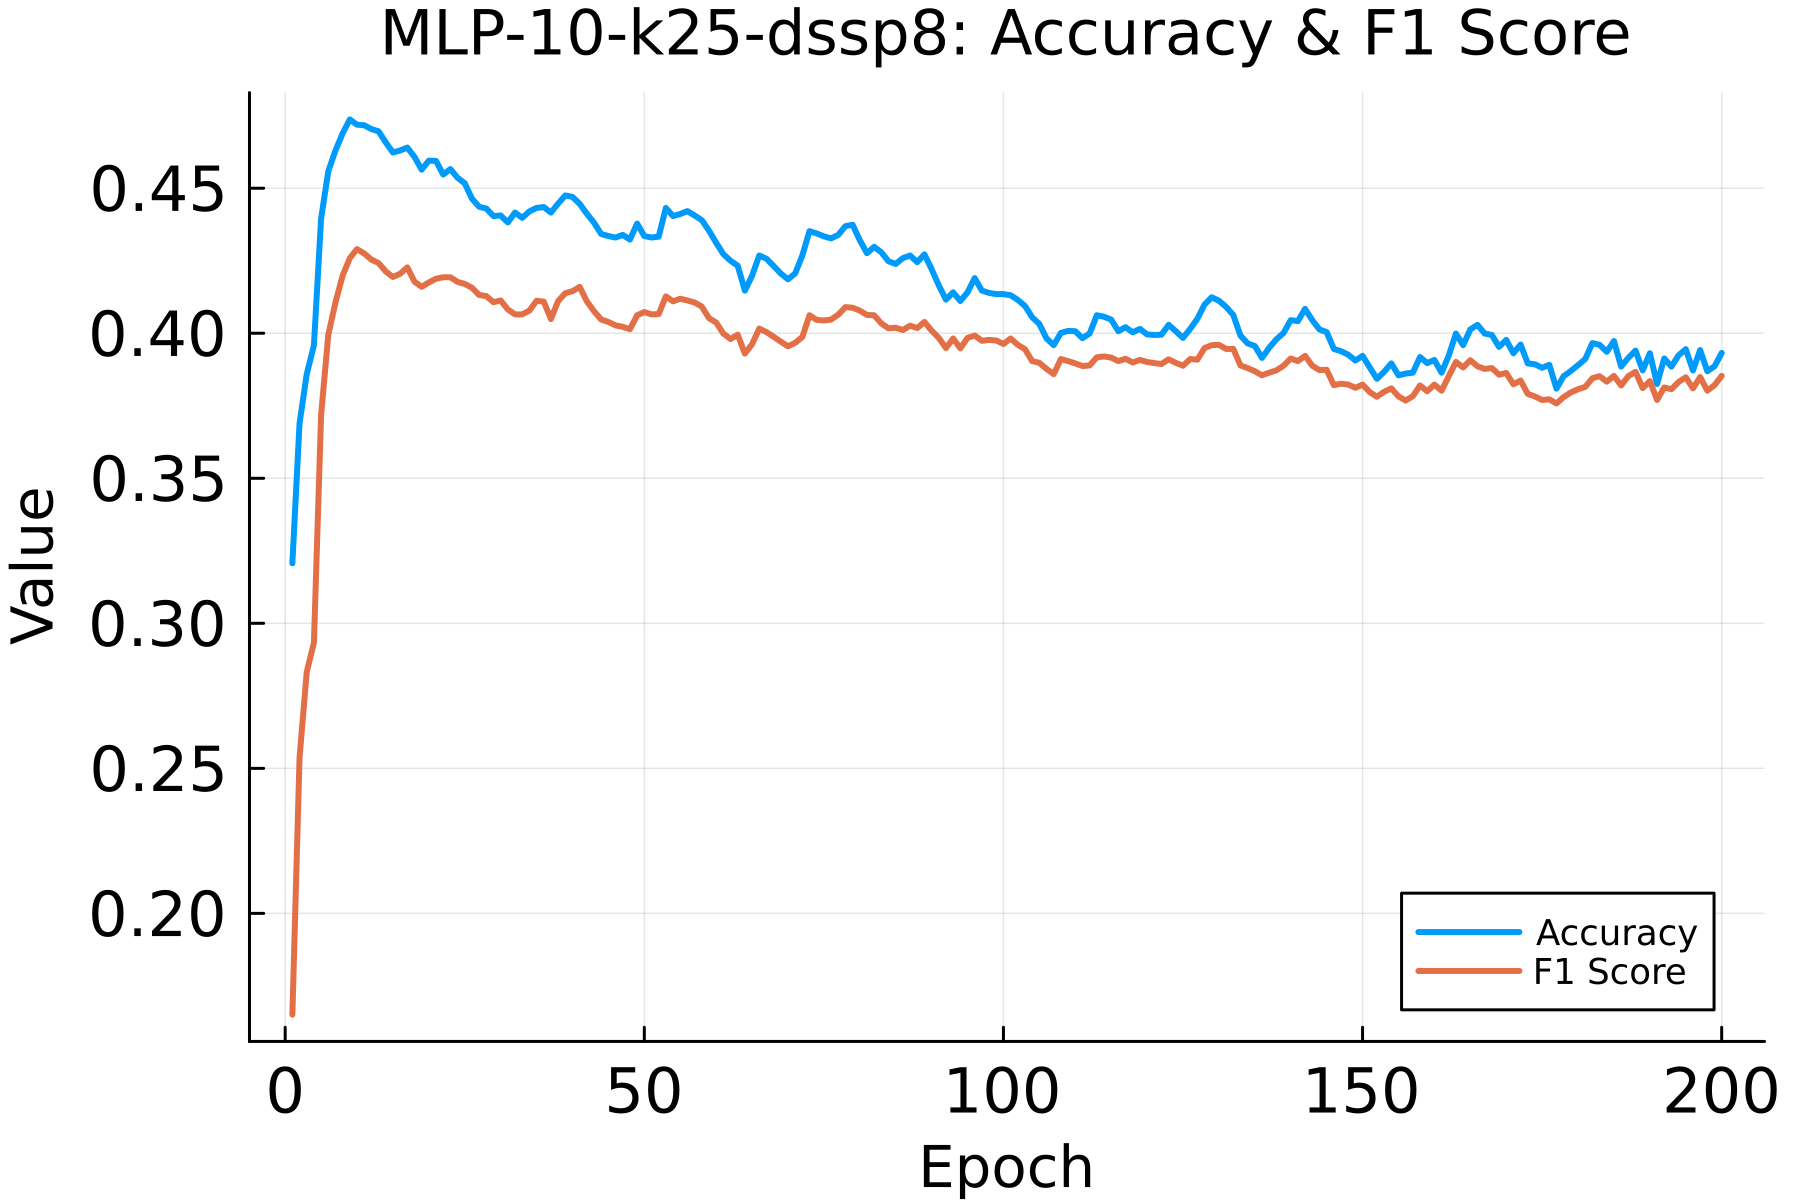
\includegraphics[width=\textwidth]{mlpfull_k25_dssp8_score}
        \label{fig:sube}
    \end{subfigure}
    
    \begin{subfigure}{0.48\textwidth}
        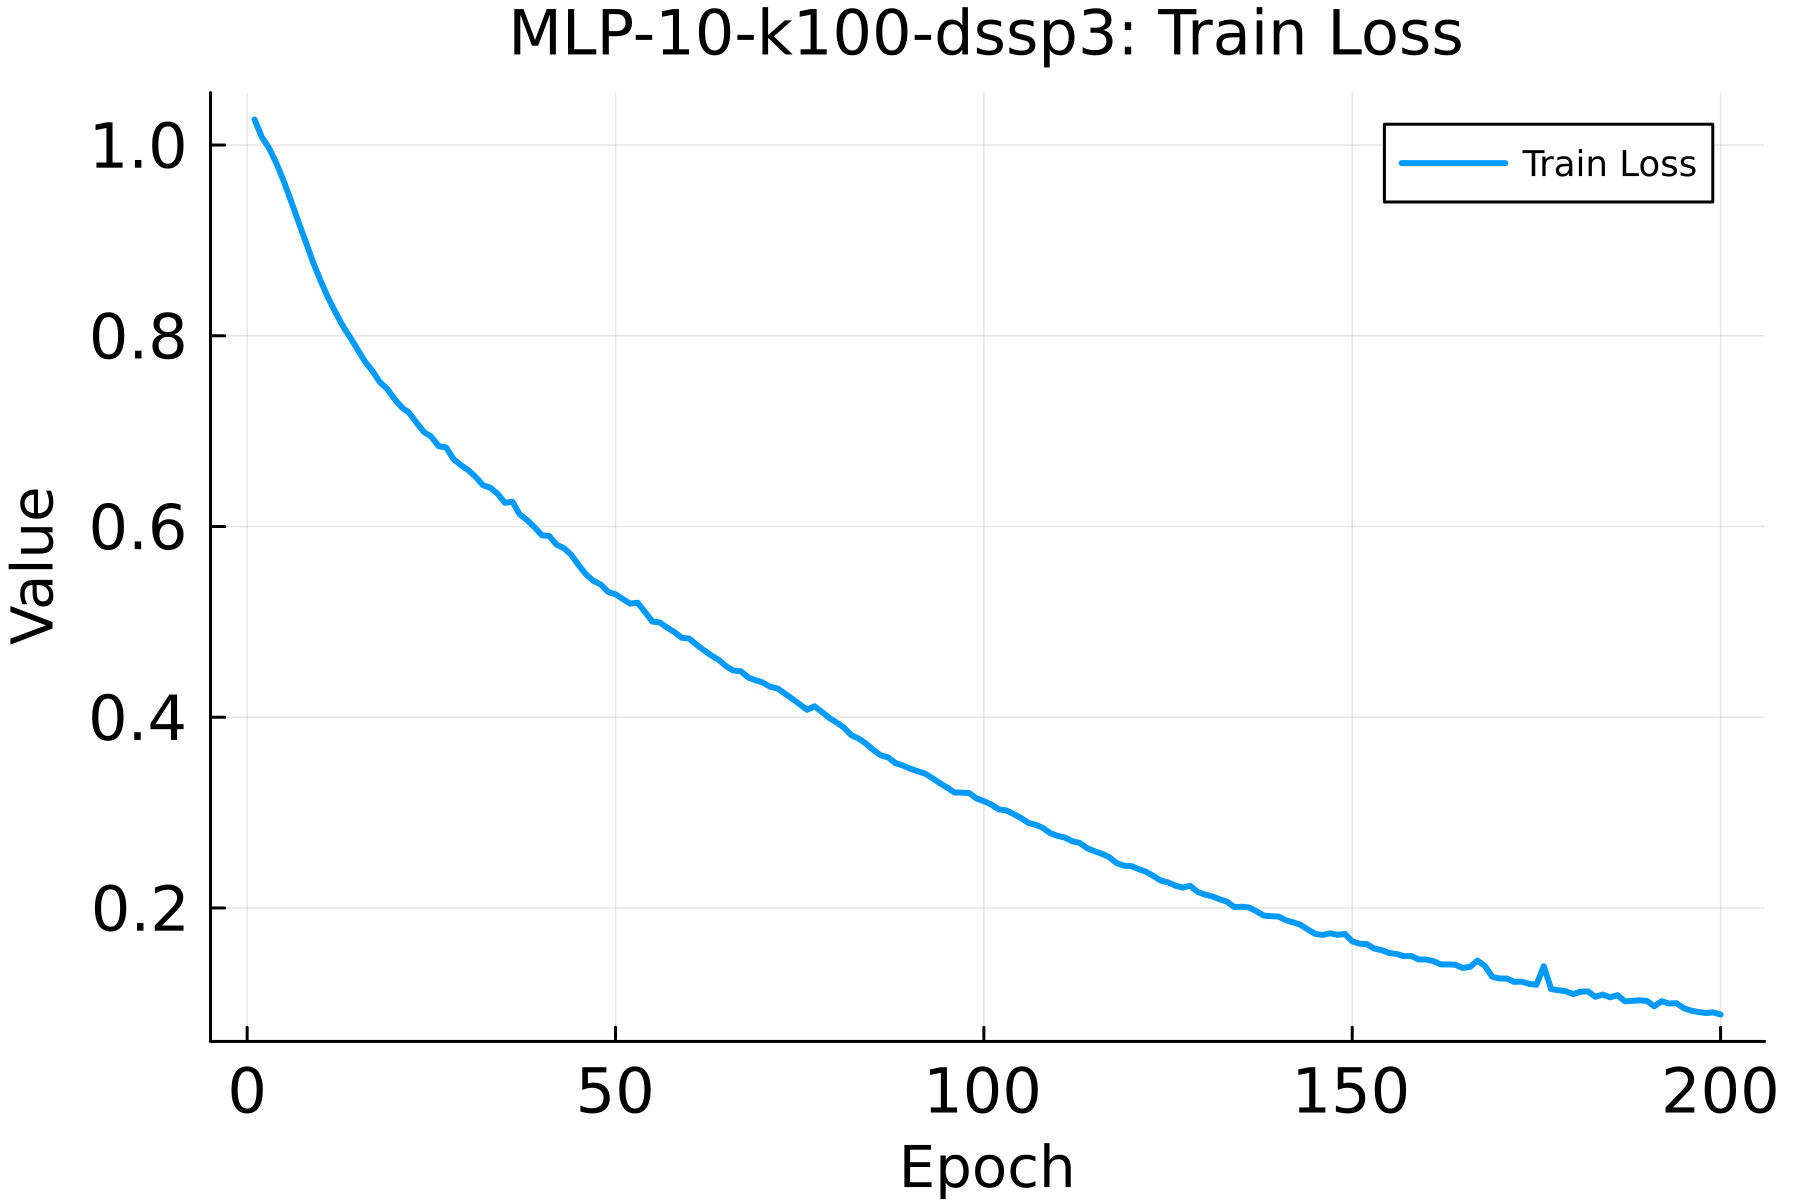
\includegraphics[width=\textwidth]{mlp_fullk100_dssp3_loss}
        \label{fig:sue}
    \end{subfigure}
    \hfill
    \begin{subfigure}{0.48\textwidth}
        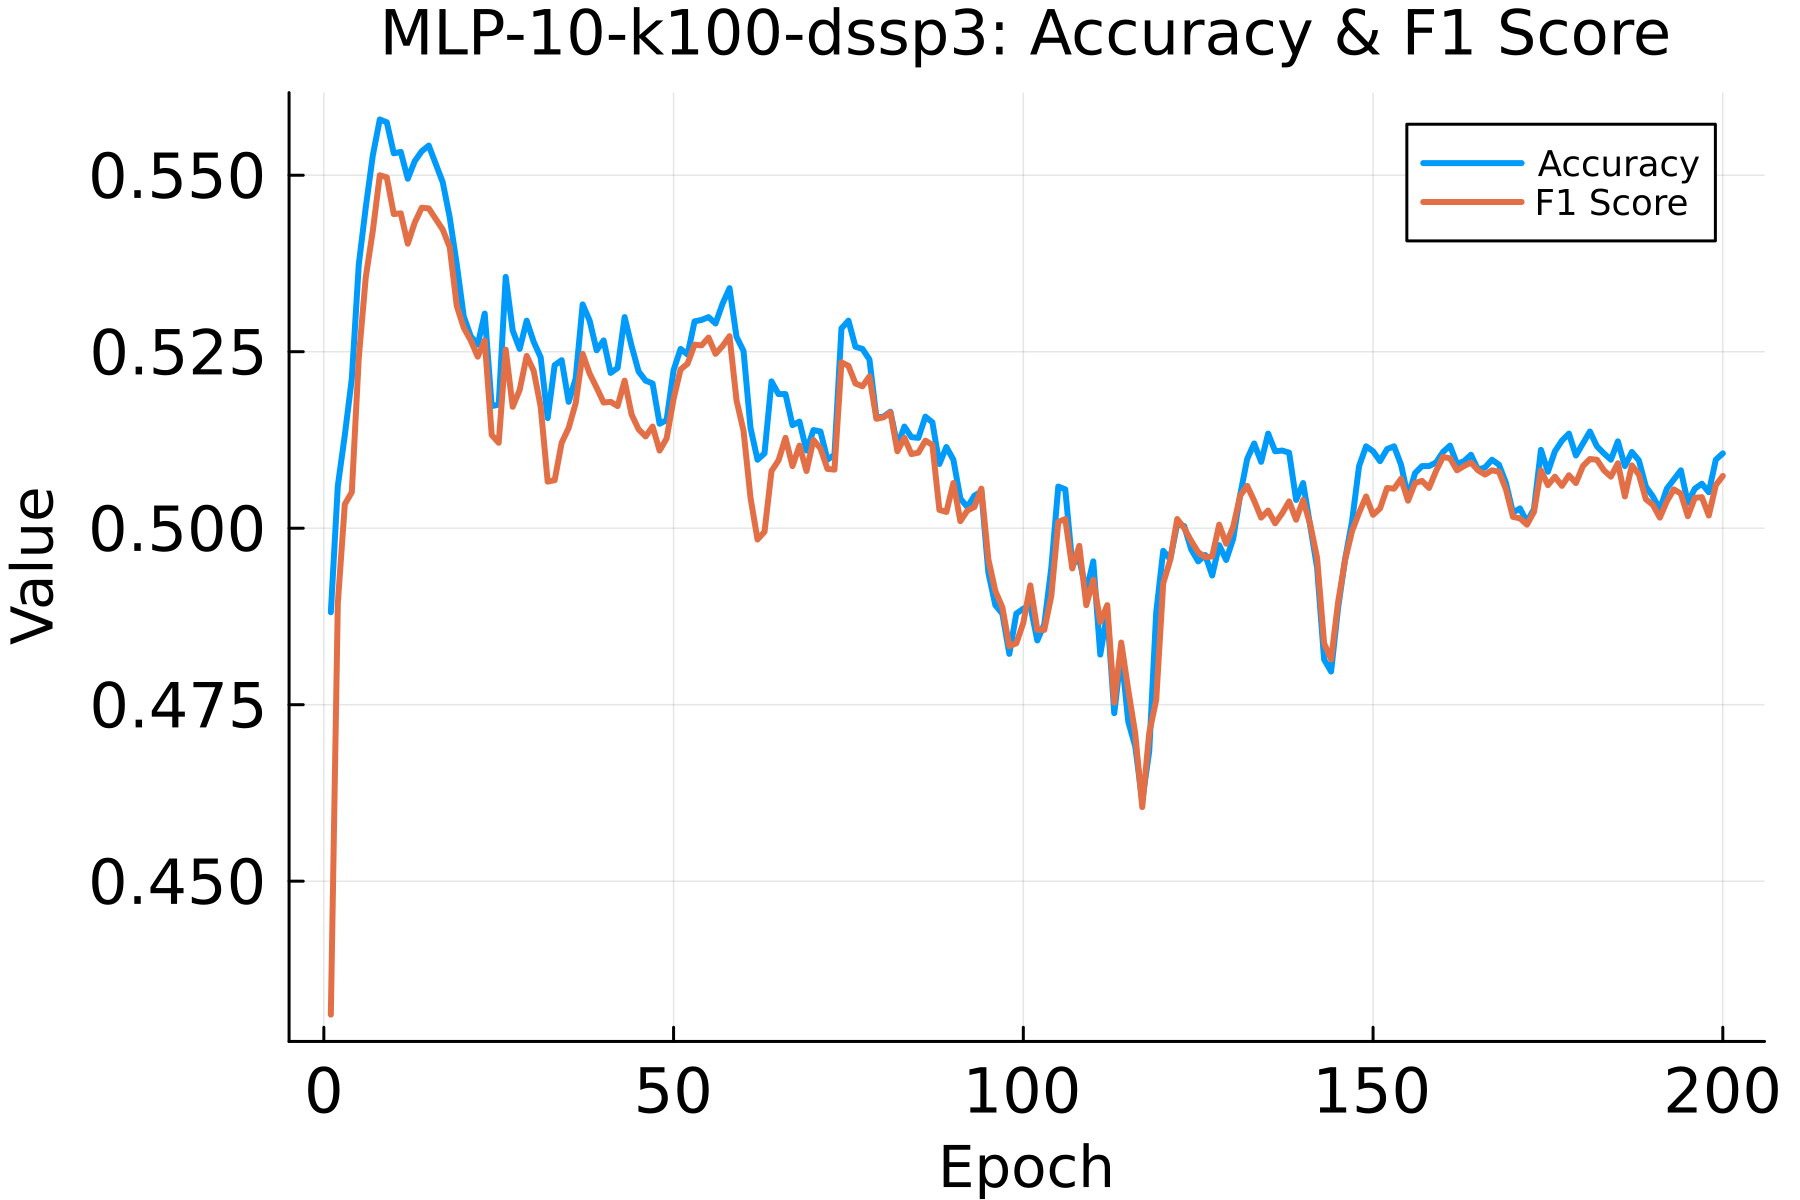
\includegraphics[width=\textwidth]{mlpfull_k100_dssp3_score}
        \label{fig:se}
    \end{subfigure}
    
    \begin{subfigure}{0.48\textwidth}
        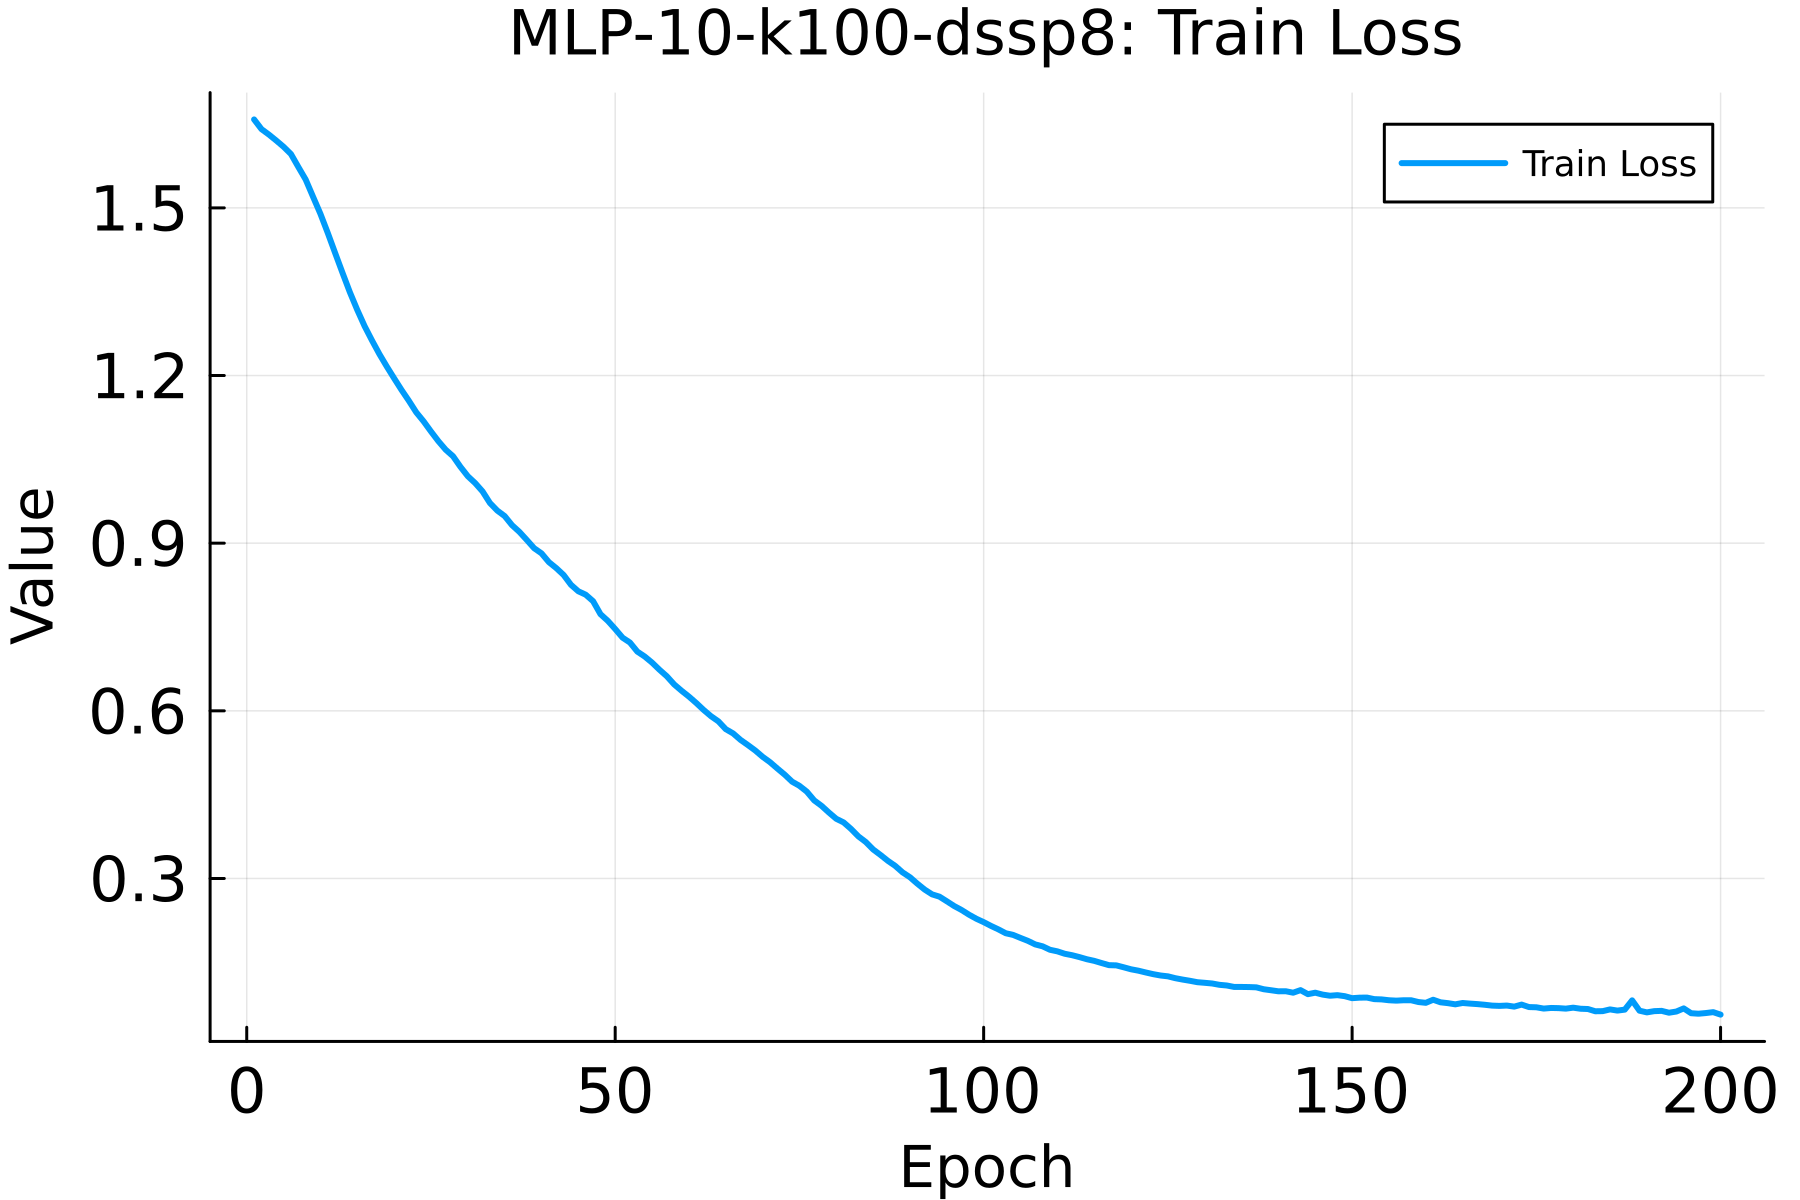
\includegraphics[width=\textwidth]{mlp_full_k100_dssp8_loss}
        \label{fig:sge}
    \end{subfigure}
    \hfill
    \begin{subfigure}{0.48\textwidth}
        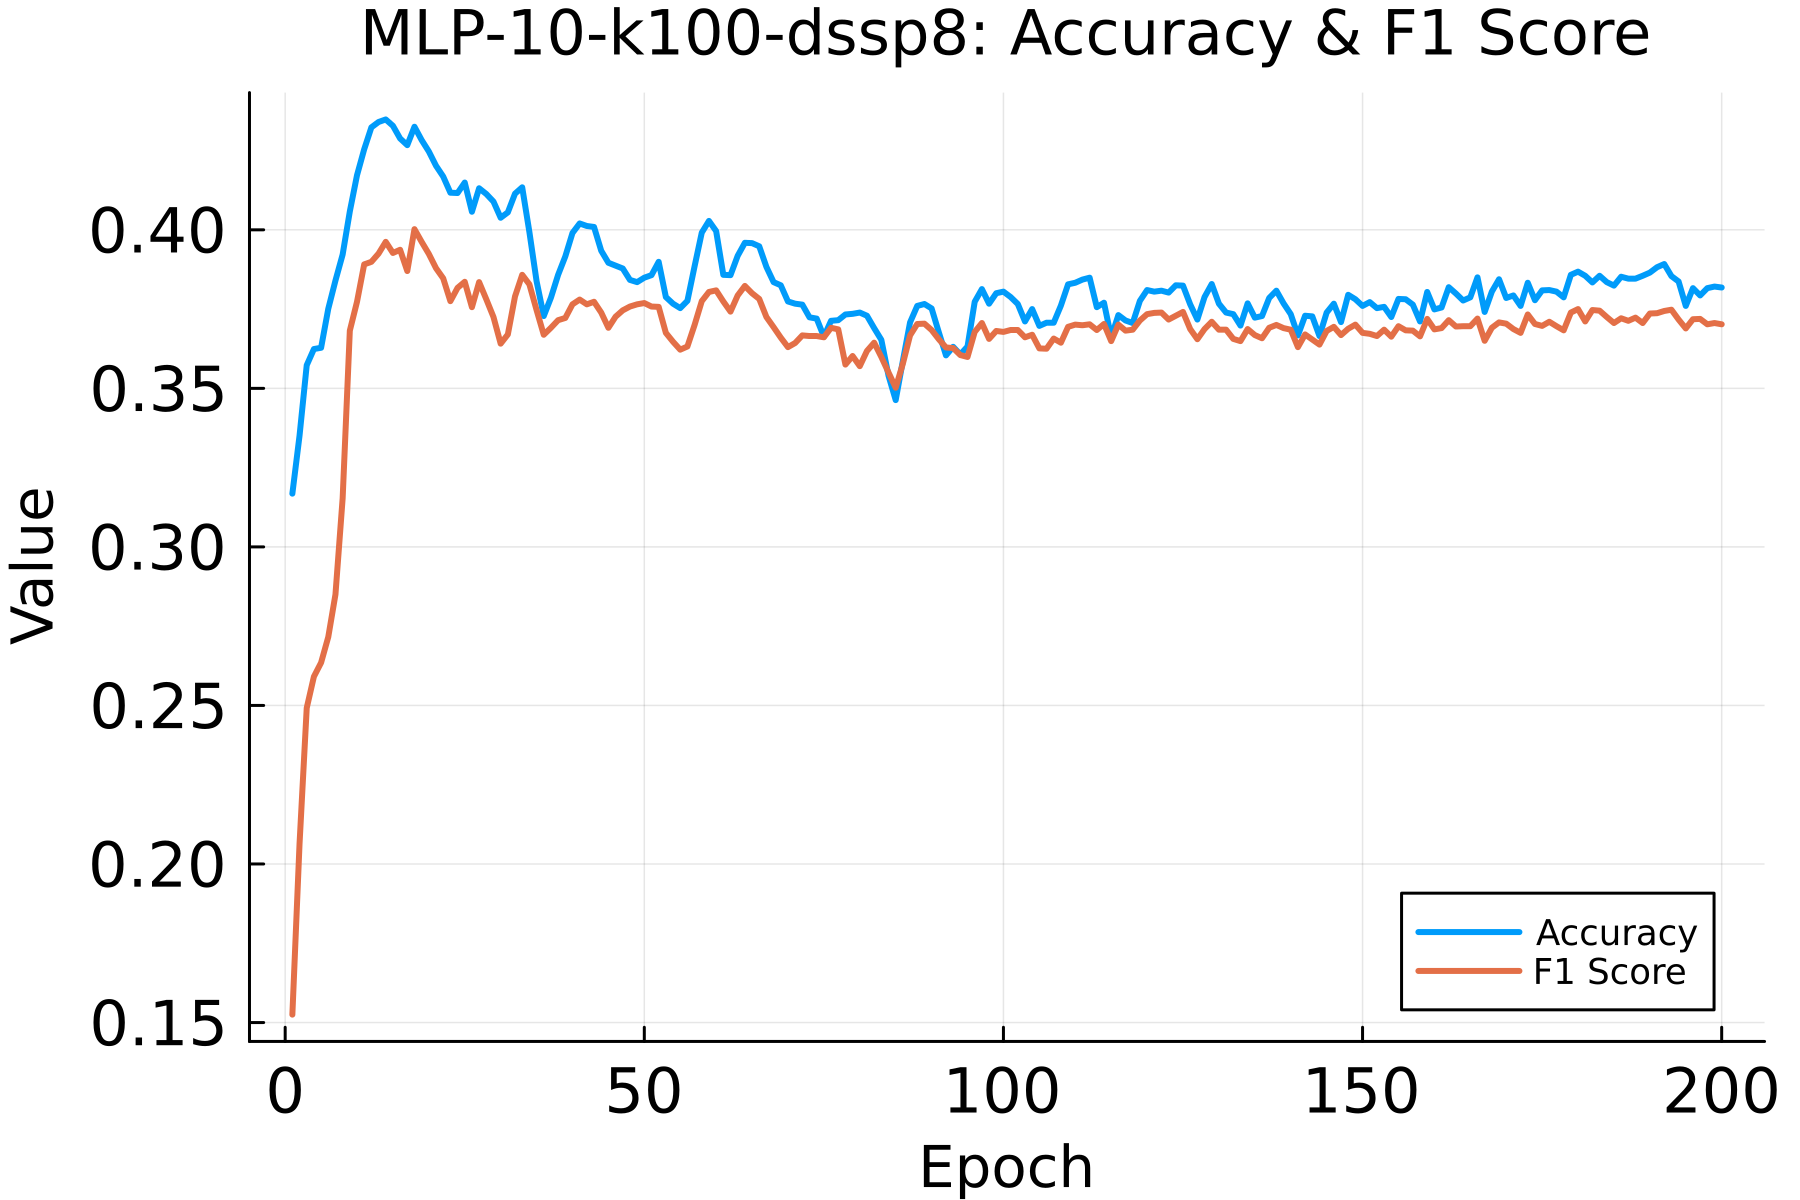
\includegraphics[width=\textwidth]{mlpfull_k100_dssp8_score}
        \label{fig:she}
    \end{subfigure}
    \caption{Performance of training procedure of the 10-layer MLP model on 60 \% of NetSurfP 2.0's training data, 0.8-0.2 training-test data split. Tested on 3 and 8 secondary structure classifications (dssp3 and dssp8 respectively) and with different kinds of hyperdimensional embeddings made with neighborhood-encoding ($n = 25$ and $n=100$).}
    \label{fig:main8e}
  \end{figure}

In contrast to the SLP and the 1-layer MLP models, the performance of the 10-layer MLP model demonstrates much more stable and consistent behavior throughout the training process, as evidenced by the performance and loss metrics, even though the resulting performance remains generally low. Although this stability may partially result from the lower learning rate, the model's computational feasibility made it an option for further investigation, prompting us to select this 133,343,733-parameter model for our subsequent tests with various datasets and comparisons with other state-of-the-art methods.

In order to benchmark our study against the capabilities of state-of-the-art protein language models, we collected the available results of other protein language models such as ESM-1b~\cite{esm}, NetSurfP 2.0~\cite{netsurf}, NetSurfP 3.0~\cite{netsurf3} and ProtTrans'~\cite{prottrans} best-performing model; ProtT5-XL-U50. ESM-1b is a model by Meta AI, trained on a large corpus of approximately 86 billion amino acid residues. It consists of around 670 million parameters and successfully utilized a transformer architecture together with evolutionary data. NetsurfP 2.0 and its successor NetSurf 3.0 are models comprising convolutional neural network (CNN) and bidirectional long short-term (biLSTM) layers. Despite being trained on a comparatively smaller dataset, they exhibit notable performance. The distinction between these two methods lies in their input configurations. ProtT5-XL-U50 is a large transformer-based model comprising 3 billion parameters, trained on UniRef50~\cite{uniref} (45 million sequences).

\begin{table}[h]
    \caption{Accuracies of secondary structure classification of a 10-layer MLP model trained on 60 \% of NetSurfP 2.0's training data encoded into different kinds of hyperdimensional embeddings made with neighborhood-encoding ($n = 25$ and $n=100$). Tested on 3 and 8 secondary structure classifications (ss3 and ss8 respectively) of the CASP12 and CB513 dataset. Performance with dummy data was also assessed.}
    \label{tab:casp}
    \centering
    \begin{tabular}{lcc|cc}
        \toprule
        \textbf{Accuracy} & CASP12 (3) & CB513 (3) & CASP12 (8) & CB513 (8)\\
        \midrule
        \textbf{ESM-1b} & 76.9 & 83.9 & 66.0 & 70.2\\
        \textbf{NetSurfP 2.0} & 82.0 & 84.5 & 66.9 & 71.3\\
        \textbf{NetSurfP 3.0} & 79.1 & 84.5 & 66.9 & 71.1\\
        \textbf{ProtT5-XL-U50} & 77.5 & 86.2 & 70.5 & 74.5\\
        \bottomrule
    \end{tabular}
  \end{table}

We evaluated the fully trained 10-layer MLP model on the test datasets, with the results summarized in Table~\ref{tab:casp}. To validate our findings, we also generated a random dummy dataset for comparison. Disappointingly, the model's performance on our test data did not surpass its performance on the randomly generated data. This may indicate that a relatively simplistic neural network is incapable of efficiently learning from high-dimensional sparse vectors. Alternatively, it may indicate that our neighborhood-encoding algorithm requires additional refinement and optimization to improve its resulting embeddings. And lastly, considering the computational limits of this study, a larger training dataset might be beneficial too.

\begin{table}[h]
    \caption{Accuracies of secondary structure classification of a 10-layer MLP model trained on 60 \% of NetSurfP 2.0's training data encoded into different kinds of hyperdimensional embeddings made with neighborhood-encoding ($n = 25$ and $n=100$). Tested on 3 and 8 secondary structure classifications (ss3 and ss8 respectively) of the CASP12 and CB513 dataset. Performance with dummy data was also assessed.}
    \label{tab:casp}
    \centering
    \begin{tabular}{lccc}
        \toprule
        \textbf{Accuracy} & CASP12 & CB513 & Random\\
        \midrule
        \textbf{n25-ss3} & 36.9 & 35.48 & 34.11\\
        \textbf{n25-ss8} & 24.88 & 21.01& 21.09\\
        \textbf{n100-ss3} & 39.33 & 37.61 & 38.74\\
        \textbf{n100-ss8} & 23.13 & 20.86 & 20.53\\
        \bottomrule
    \end{tabular}
  \end{table}

  \begin{table}[h]
    \caption{F1-scores of secondary structure classification of a 10-layer MLP model trained on 60 \% of NetSurfP 2.0's training data encoded into different kinds of hyperdimensional embeddings made with neighborhood-encoding ($n = 25$ and $n=100$). Tested on 3 and 8 secondary structure classifications (ss3 and ss8 respectively) of the CASP12 and CB513 dataset. Performance with dummy data was also assessed.}
    \label{tab:casp2}
    \centering
    \begin{tabular}{lccc}
        \toprule
        \textbf{Accuracy/F1} & CASP12 & CB513 & Random\\
        \midrule
        \textbf{n25-ss3} & 37.50 & 35.52 & 34.35\\
        \textbf{n25-ss8} & 18.61 & 15.30 & 14.79\\
        \textbf{n100-ss3} & 37.19 & 35.68 & 36.07\\
        \textbf{n100-ss8} & 20.25 & 18.03 & 17.80\\
        \bottomrule
    \end{tabular}
  \end{table}